\documentclass[]{book}
\usepackage{lmodern}
\usepackage{amssymb,amsmath}
\usepackage{ifxetex,ifluatex}
\usepackage{fixltx2e} % provides \textsubscript
\ifnum 0\ifxetex 1\fi\ifluatex 1\fi=0 % if pdftex
  \usepackage[T1]{fontenc}
  \usepackage[utf8]{inputenc}
\else % if luatex or xelatex
  \ifxetex
    \usepackage{mathspec}
  \else
    \usepackage{fontspec}
  \fi
  \defaultfontfeatures{Ligatures=TeX,Scale=MatchLowercase}
\fi
% use upquote if available, for straight quotes in verbatim environments
\IfFileExists{upquote.sty}{\usepackage{upquote}}{}
% use microtype if available
\IfFileExists{microtype.sty}{%
\usepackage{microtype}
\UseMicrotypeSet[protrusion]{basicmath} % disable protrusion for tt fonts
}{}
\usepackage{hyperref}
\hypersetup{unicode=true,
            pdftitle={Aging Well Lab Manual},
            pdfauthor={Kendra Seaman},
            pdfborder={0 0 0},
            breaklinks=true}
\urlstyle{same}  % don't use monospace font for urls
\usepackage{natbib}
\bibliographystyle{apalike}
\usepackage{longtable,booktabs}
\usepackage{graphicx,grffile}
\makeatletter
\def\maxwidth{\ifdim\Gin@nat@width>\linewidth\linewidth\else\Gin@nat@width\fi}
\def\maxheight{\ifdim\Gin@nat@height>\textheight\textheight\else\Gin@nat@height\fi}
\makeatother
% Scale images if necessary, so that they will not overflow the page
% margins by default, and it is still possible to overwrite the defaults
% using explicit options in \includegraphics[width, height, ...]{}
\setkeys{Gin}{width=\maxwidth,height=\maxheight,keepaspectratio}
\IfFileExists{parskip.sty}{%
\usepackage{parskip}
}{% else
\setlength{\parindent}{0pt}
\setlength{\parskip}{6pt plus 2pt minus 1pt}
}
\setlength{\emergencystretch}{3em}  % prevent overfull lines
\providecommand{\tightlist}{%
  \setlength{\itemsep}{0pt}\setlength{\parskip}{0pt}}
\setcounter{secnumdepth}{5}
% Redefines (sub)paragraphs to behave more like sections
\ifx\paragraph\undefined\else
\let\oldparagraph\paragraph
\renewcommand{\paragraph}[1]{\oldparagraph{#1}\mbox{}}
\fi
\ifx\subparagraph\undefined\else
\let\oldsubparagraph\subparagraph
\renewcommand{\subparagraph}[1]{\oldsubparagraph{#1}\mbox{}}
\fi

%%% Use protect on footnotes to avoid problems with footnotes in titles
\let\rmarkdownfootnote\footnote%
\def\footnote{\protect\rmarkdownfootnote}

%%% Change title format to be more compact
\usepackage{titling}

% Create subtitle command for use in maketitle
\providecommand{\subtitle}[1]{
  \posttitle{
    \begin{center}\large#1\end{center}
    }
}

\setlength{\droptitle}{-2em}

  \title{Aging Well Lab Manual}
    \pretitle{\vspace{\droptitle}\centering\huge}
  \posttitle{\par}
    \author{Kendra Seaman}
    \preauthor{\centering\large\emph}
  \postauthor{\par}
      \predate{\centering\large\emph}
  \postdate{\par}
    \date{2019-09-06}

\usepackage{booktabs}
\usepackage{amsthm}
\makeatletter
\def\thm@space@setup{%
  \thm@preskip=8pt plus 2pt minus 4pt
  \thm@postskip=\thm@preskip
}
\makeatother

\begin{document}
\maketitle

{
\setcounter{tocdepth}{1}
\tableofcontents
}
\hypertarget{introduction}{%
\chapter{Introduction}\label{introduction}}

Welcome to the Aging Well Lab manual! This manual was created by the Lab Director, Kendra Seaman, to convey my vision for our lab and to communicate community expectations. This manual will be updated regularly as our lab grows and develops. If you have any comments or suggestions regarding the content of this manual, please share these with me. This is a living document and will change as needed.

Since we are a brand-new lab, this manual was inspired by (and in some places directly copied from) other lab manuals, including \href{https://github.com/memobc/memolab-manual}{MemoLab Manual}, \href{http://jpeelle.net/peellelab_manual.pdf}{Peele Lab Manual}, and \href{https://github.com/DVSneuro/smithlab_manual/blob/master/SmithLab_manual.pdf}{Smith Lab Manual}. Thanks to everyone who has shared their resources!

\hypertarget{about-the-lab}{%
\section{About the Lab}\label{about-the-lab}}

Our research is dedicated to using basic and translational scientific research to promote health and wellbeing across adulthood. We use a variety of behavioral, modeling and neuroimaging techniques to better understand how the mind and the brain change as people get older.

\textbf{Address:}\\
Aging Well Laboratory\\
Center for Vital Longevity\\
1600 Viceroy Drive, Suite 800\\
Dallas, TX 75235


\includegraphics{images/cvl.jpg}

\hypertarget{lab-info}{%
\section{Lab Info}\label{lab-info}}

The lab has several public-facing accounts that anyone can access:

\begin{itemize}
\tightlist
\item
  Website: \url{https://agingwelllab.github.io/}
\item
  GitHub: \url{https://github.com/agingwelllab}
\item
  OSF: \url{https://osf.io/26jqs/}
\end{itemize}

The lab also has sites that are only accessible to lab members:

\begin{itemize}
\tightlist
\item
  CVL Lab Wiki: \url{https://cvlwiki.utdallas.edu/doku.php?id=seamanlab:home}
\item
  Asana: \url{https://app.asana.com}
\item
  Slack: \url{https://agingwelllab.slack.com}
\end{itemize}

\hypertarget{approach}{%
\chapter{Approach}\label{approach}}

We use cognitive modeling and neuroimaging to understand how people learn and make decisions. We are interested how these processes \emph{do, or do not,} change as people get older. The ultimate goal of this research is to promote health and wellbeing across adulthood.


\includegraphics{images/xkcd_science.png}

Recognize that this work is inherently interdisciplinary, meaning we will use tools and knowledge from traditional fields like psychology, neuroscience, and economics. Because it requires competency in so many different domains, the learning curve can be steep and can feel overwhelming - but this is also what makes it interesting and rewarding work. Hang in there. It will get easier.

\hypertarget{mentorship-and-idps}{%
\section{Mentorship and IDPs}\label{mentorship-and-idps}}

To help you with this endeavor, you will be assigned a mentor within the lab. If you are a lab manager, graduate student, or postdoc, the Lab Director will likely be your mentor. If you are an undergraduate, you will likely be reporting to the lab manager, a graduate student, or a postdoc. To facilitate these relationships, we will use individual development plans (IDPs). The structure of IDPs will vary depending on your role in the lab, but generally they will set and track short-term and long-term goals. These will be created when you join the lab and be revisited each semester (i.e.~Fall, Spring, and Summer).

\hypertarget{feedback}{%
\section{Feedback}\label{feedback}}

You should expect to regularly receive feedback from your mentor and your peers. Feedback, especially negative feedback, can be discouraging and overwhelming. Please recognize that the purpose of feedback is to improve your work and help you meet your goals. Also know that giving critical and constructive feedback is an time-consuming effort and \textbf{try} to accept feedback in the spirit in which it is offered. As a group, we will discuss how to give and receive feedback.


\includegraphics{images/i-love-feedback.jpg}

\hypertarget{code-of-conduct}{%
\chapter{Code of Conduct}\label{code-of-conduct}}

All lab members are expected to agree with the following code of conduct. We will enforce this code as needed. We expect cooperation with all members to help ensure a safe environment for everyone. Please also see the \href{https://policy.utdallas.edu/utdbp3090}{UT Dallas Nondiscrimination policy}.

\hypertarget{the-quick-version}{%
\subsection{The Quick Version}\label{the-quick-version}}

The Aging Well Lab is committed to providing a harrassment-free environment, regardless of gender, gender identity and expression, age, sexual orientation, disability, physical appearance, body size, race, or religion (or lack thereof). We do not tolerate harrassment of lab members in any form. Sexual language and imagery is generally not appropriate for any lab venue, including lab meetings, presentations, or discussions.

\hypertarget{the-less-quick-version}{%
\subsection{The Less Quick Version}\label{the-less-quick-version}}

Harassment includes offensive verbal comments related to gender, gender identity and expression, age, sexual orientation, disability, physical appearance, body size, race, religion, sexual images in public spaces, deliberate intimidation, stalking, following, harassing photography or recording, sustained disruption of talks or other events, inappropriate physical contact, and unwelcome sexual attention.

Members asked to stop any harassing behavior are expected to comply immediately.

If you are being harassed, notice that someone else is being harassed, or have any other concerns, please contact Kendra Seaman immediately. If Kendra is the cause of your concern, then please reach out to one of the center directors or another trusted departmental member who can assist.

We expect members to follow these guidelines at any lab-related event.

This section was adapted from the \href{https://github.com/memobc/memolab-manual\#code-of-conduct}{MemoLab}.

\hypertarget{expectations-and-responsibilities}{%
\chapter{Expectations and Responsibilities}\label{expectations-and-responsibilities}}

\hypertarget{everyone}{%
\section{Everyone}\label{everyone}}

\hypertarget{big-picture}{%
\subsection{Big Picture}\label{big-picture}}

We expect everyone to:

\begin{itemize}
\tightlist
\item
  \textbf{Be supportive} - We're all in this together!\\
\item
  \textbf{Share your knowledge.} Mentorship takes many forms, but frequently involves looking out for those who are more junior to us. If you've done something before, share your experience. We are a team and we should work together.
\item
  \textbf{Be engaged in the community.}

  \begin{itemize}
  \tightlist
  \item
    Attend and actively engage in lab and one-on-one meetings. Ask questions, make suggestions, etc. If you are easily distracted by technology, disconnect during meetings.\\
  \item
    Attend talks in the CVL, BBS, and greater UTD community.\\
  \item
    Be an positive representative and advocate for our lab and our lab's work in our larger research communities.
  \end{itemize}
\end{itemize}

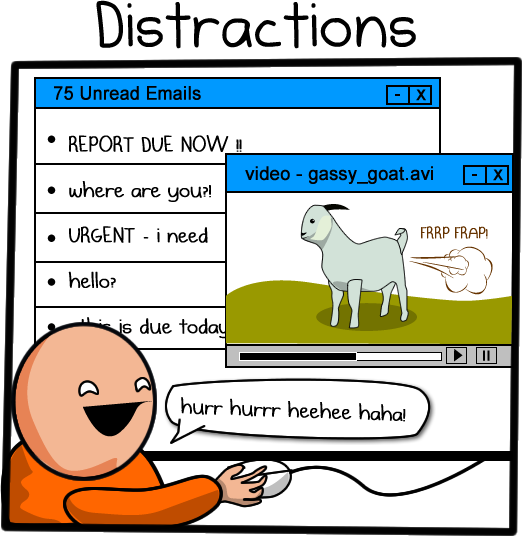
\includegraphics{images/distractions.png}

\begin{itemize}
\tightlist
\item
  Be independent when possible, ask for help when necessary. Specifically, ask three, then me!

  \begin{itemize}
  \tightlist
  \item
    There are lots of web resources you should consult - StackOverflow, NeuroStars, etc\\
  \item
    Use others in the lab (and in the CVL, BBS) and external collaborators.\\
  \end{itemize}
\item
  \textbf{Communicate honestly}, even when it's difficult.\\
\item
  Do work we are proud of individually and as a group.

  \begin{itemize}
  \tightlist
  \item
    Double check your work.\\
  \item
    Our lab has a commitment to open science. Be ready to share your work both within the lab and with outsides at the conclusion of a project.
  \end{itemize}
\item
  Work towards proficiency in Unix, BASH, R, and Python.
\item
  Respect each other's strengths, weaknesses, differences, and beliefs.

  \begin{itemize}
  \tightlist
  \item
    Be patient with everyone (including the Lab Director). Most of us are learning new skills and are busier than we would like.
  \end{itemize}
\item
  Adhere to the ethical principles as described by the \href{https://www.apa.org/ethics/code/}{Association for Psychological Science}, \href{https://www.sfn.org/Membership/Professional-Conduct/SfN-Ethics-Policy}{Society for Neuroscience}, and \href{https://research.utdallas.edu/orio/rcr}{UT Dallas Responsible Conduct of Research}.
\item
  Maintain a professional and accurate online presence. Make sure you keep your online profiles up to date. Remember, we all represent the lab and the lab represents us.
\end{itemize}

\hypertarget{small-picture}{%
\subsection{Small Picture}\label{small-picture}}

We're sharing a relatively small space, so please be thoughtful of others. Specifically:

\begin{itemize}
\tightlist
\item
  \textbf{Do not come into the lab if you are sick!} It's better to keep everyone healthy. If you are sick, email your mentor and the lab manager.
\end{itemize}


\includegraphics{images/sick.jpg}

\begin{itemize}
\tightlist
\item
  Keep the lab neat.

  \begin{itemize}
  \tightlist
  \item
    Do not leave food, drinks, or crumbs in the lab.\\
  \item
    Items left unattended may be cleaned, reclaimed or recycled.
  \end{itemize}
\end{itemize}

\hypertarget{lab-director}{%
\section{Lab Director}\label{lab-director}}

As the lab director, you can expect me to:

\begin{itemize}
\tightlist
\item
  Have a vision for where the lab is going, both in the short-term (next few weeks) and in the long-term (next few years).
\item
  Obtain funding to support our laboratory.\\
\item
  Care about your happiness.
\item
  Support your career development, including:

  \begin{itemize}
  \tightlist
  \item
    writing recommendation letters,\\
  \item
    introducing you to other scientists (potential future mentors and colleagues),\\
  \item
    promoting your work as often as possible (at conferences),\\
  \item
    facilitating conference travel (see position-dependent specifics below), and\\
  \item
    working with mentees (Postdocs, Mentees) to create an Individual Development Plan (IDP).\\
  \end{itemize}
\item
  Support your personal development, including:

  \begin{itemize}
  \tightlist
  \item
    flexible working hours and environment (when feasible), and\\
  \item
    encouraging activities outside of school/work.\\
  \end{itemize}
\item
  Make the time to meet with you regularly, read and provide feedback on code, posters, manuscripts, and other data products.
\item
  Obsess over chosing the correct analyses, clear phrasing, and awesome data visualizations.
\end{itemize}


\includegraphics{images/boss.jpg}

\hypertarget{employees}{%
\section{Employees}\label{employees}}

Employee salaries follow the \href{https://www.utdallas.edu/hr/compensation/classified/}{UTD paygrade}.

\hypertarget{lab-manager}{%
\subsection{Lab Manager}\label{lab-manager}}

The lab manager is the heart and soul of the lab. While other lab members (including the Lab Director) may have flexible or irregular schedules, the lab manager will be a constant presence for the lab in the Center for Vital Longevity (CVL).

In order to provide constency for the lab, I expect the lab manager to:

\begin{itemize}
\tightlist
\item
  maintain regularly scheduled hours on weekdays (except for \href{https://www.utdallas.edu/hr/news/holidays/}{UTD holidays}),\\
\item
  serve as a liason between the the CVL administrative staff and our lab,\\
\item
  check the lab email and personal work email accounts daily and respond to all emails within two business days, and\\
\item
  check the voicemail daily and arrange for return calls to be made within one business day.
\end{itemize}


\includegraphics{images/email.png}

The Lab Manager's primary responsibilities include:

\begin{itemize}
\tightlist
\item
  facilitating the purchase and setup of any new equipment for the lab,\\
\item
  coordinating and training all lab research assistants,\\
\item
  assisting with the design and implementation of behavioral, eye-tracking, and fMRI experiments,\\
\item
  overseeing the recruitment and testing of study participants, and\\
\item
  helping with preprocessing and analysis of experimental data.
\end{itemize}

\hypertarget{paid-post-bacc-research-assistants}{%
\subsection{Paid post-bacc Research Assistants}\label{paid-post-bacc-research-assistants}}

TBD

\hypertarget{postdocs-and-staff-scientists}{%
\subsection{Postdocs and Staff Scientists}\label{postdocs-and-staff-scientists}}

I will expect postdocs and staff scientists to move towards being more PI-like, including:

\begin{itemize}
\tightlist
\item
  giving conference talks,\\
\item
  writing grant proposals, and\\
\item
  cultivating an independent research program (up to 10\% of time).
\end{itemize}

Also, to have (or acquire) the technical and open science skills listed for PhD students below.

\includegraphics{images/postdoc.gif}

Postdoc salaries generally follow \href{https://www.niaid.nih.gov/grants-contracts/salary-cap-and-stipend-levels-announced}{NIH guidelines}.

\hypertarget{students}{%
\section{Students}\label{students}}

\hypertarget{phd-students}{%
\subsection{PhD Students}\label{phd-students}}

I will expect graduate students to:

\begin{itemize}
\tightlist
\item
  attend classes, colloquium, and relevant talks around campus,\\
\item
  be \textbf{excited} about the research questions they are asking, be \textbf{eager} to find the answers, and \textbf{anxious} to share their results with others,
\end{itemize}


\includegraphics{images/bestdata.jpeg}

\begin{itemize}
\tightlist
\item
  seek out and apply for fellowships and awards (including travel awards), and\\
\item
  realize there are times for pulling all-nighters and times for smelling the roses.
\end{itemize}

I will expect graduate students to move towards:

\begin{itemize}
\tightlist
\item
  expertise in their chosen field(s) by knowing the literature like the back of their hand (see below for suggestions on how to do this),
\item
  proficiency in using R and/or Python for data analysis and model fitting,
\item
  writing BASH shell scripts for imaging analysis in FSL,
\item
  sharing your work with me (and others) using R Markdown and/or Jupyter notebooks,
\item
  preregistering their experiments publicly on OSF,
\item
  sharing their data and scripts publicly on OSF and/or GitHub,
\item
  making figures and posters using R or Python along with Adobe Illustrator,
\item
  clearly communicating your results in written and verbal formats, and
\item
  actively mentoring those working for them (undergraduate RAs), including completing an Individual Development Plan (IDP).
\end{itemize}

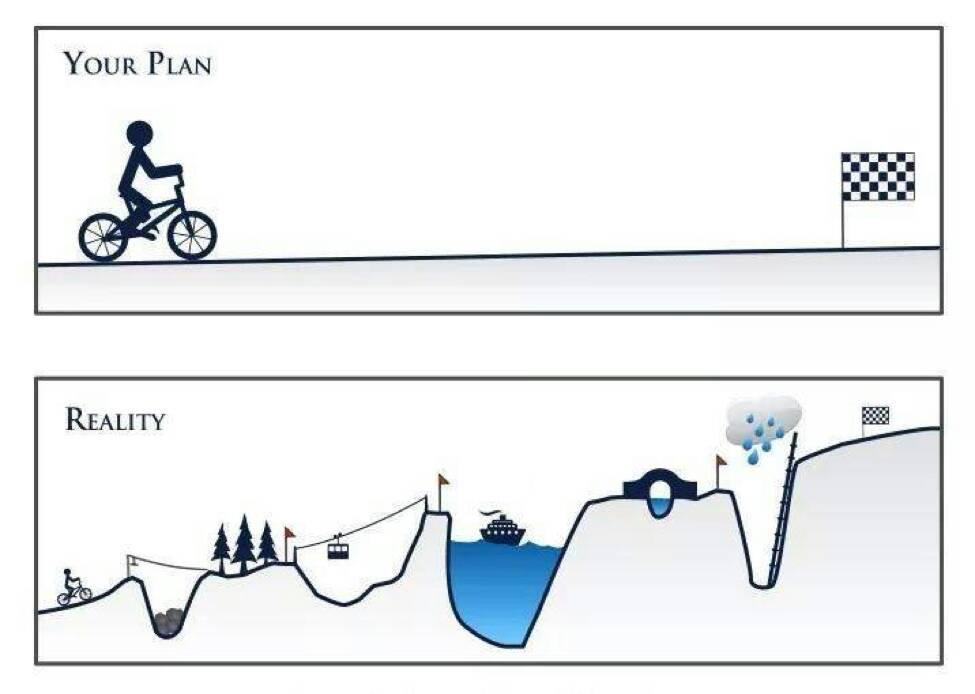
\includegraphics{images/phdplan.jpg}

The learning curve for these skills can be steep, but developing these skills is necessary for success in both cognitive neuroscience and data science. If these goals do not align with your own interests and goals, then my lab is probably not a good fit for you.

\hypertarget{masters-students}{%
\subsection{Master's Students}\label{masters-students}}

I will expect Master's students to move towards being more PhD student-like. In particular, by the end of their time in the lab, I expect master's students to:\\
* complete an empirical study in the lab, and\\
* complete a poster and/or written manuscript of that study.


\includegraphics{images/researchcat.jpg}

\hypertarget{undergraduate-students}{%
\subsection{Undergraduate Students}\label{undergraduate-students}}

Undergraduate students will play a vital role in our lab. Students can be involved in the lab in a number of ways, including independent study projects, student works, and internships. Given that we have limited time and resources, unfortunately we cannot accept or keep all undergraduates who are interested in our lab. Based on the lab's needs, we will consider new undergraduates at the beginning of each term. Each new undergraduate must attend a manditory orientation session, journal club, and serve a probationary term (one semester) before advancing further in the lab.


\includegraphics{images/RAmeme.jpg}

I expect undergraduates to:

\begin{itemize}
\tightlist
\item
  commit to work \emph{at least} 5 hours per week in the lab and maintaining those hours on the lab calendar,
\item
  show up on time for meetings, lab hours, and testing,\\
\item
  make sure all of your work is accurate (double-check everything), and
\item
  be willing to help with whatever projects need it.
\end{itemize}

In most cases, undergraduates will be directly mentored by the lab manager for their first semester in the lab, and then move on to work directly with a research assistant or graduate student.

\hypertarget{communication}{%
\chapter{Communication}\label{communication}}


\includegraphics{images/communication.png}

Communication is critical. Whether you pursue academia or industry, you will need to be able to communicate with others about your work. We will likely have to go beyond memes in order to do this.

\hypertarget{lab-meetings}{%
\section{Lab Meetings}\label{lab-meetings}}

Regular lab meetings are essential for making sure that we move both current and future projects forward. They also help us function as a team. We will use lab meetings to discuss administrative and practical issues, solicit feedback on current analyses and code, discuss current literature, and practice conference and job talks. Our weekly lab meetings will run approximately 1-1.5 hours long. All full-time staff and graduate students will be expected to attend (unless cleared with the Lab Director in advance).

During lab meetings, one or two presenters will be responsible for setting the agenda that day. The presenter/s will also be responsible for sharing any relevant materials (e.g.~journal article) a couple of days in advance. If you're scheduled to present and need to cancel or postpone, please give the group 72 hours notice. \textbf{Everyone is expected to participate in lab meetings.} That means reading relevant material beforehand and if you are easily distracted by your computer or phone, put it away.


\includegraphics{images/labmeeting.gif}

\hypertarget{individual-meetings}{%
\section{Individual Meetings}\label{individual-meetings}}

All mentors should have weekly meetings with their mentees, lasting between 15 minutes to an hour. For instance, as lab director, I will have weekly meetings with the lab manager, postdocs, staff scientists, and any students leading projects. Ideally, the agenda for these meetings should be set by the mentee; you should provide a quick overview of the progress you've made on your project and let your mentor know where you're stuck and/or need help. You can also use individual meetings to seek feedback about new project development or professional development.


\includegraphics{images/best_meeting.jpg}

\hypertarget{asana}{%
\section{Asana}\label{asana}}

Asana is a project-management platform that we will use to track progress on various projects in the lab.

\begin{itemize}
\tightlist
\item
  Asana is basically an orgnaized to-do list. When adding a task, make sure to put a useful description, assign it to someone and set a tentative due date.\\
\item
  Be realistic and flexible with due dates. Of course you should try to get things done in a timely manner, but sometimes, life happens and you have to adjust.\\
\item
  If you're leading a project in the lab, please make sure that your project is listed on Asana. All project-related tasks should be under your project.
\end{itemize}


\includegraphics{images/asana.jpg}

\hypertarget{slack}{%
\section{Slack}\label{slack}}

Slack is a team-collaboration tool that we will use for communication.

\begin{itemize}
\tightlist
\item
  Try to avoid direct messages in Slack. Instead, find a home for your comment or question in an existing channel. This allows you to get answers and feedback from multiple people in the lab.\\
\item
  When replying to a question or comment, try to use threads. This keeps the conversation organized and easy to navigate.
\end{itemize}


\includegraphics{images/slack.png}

\hypertarget{email}{%
\section{Email}\label{email}}

When contacting me, please use Slack (or Asana) whenever possible. I will try to respond to emails, but please don't use it for anything urgent.


\includegraphics{images/email2.jpeg}

Likewise, I will try to use Asana/Slack to communicate with you as much as possible. However, sometimes I will need to email you. \textbf{I expect you will read all email sent to you and respond (if a response is needed) within one business day.} If you will not be checking email for more than a couple of days, please consider using a vacation message so that others know you are not available on email (this suggestion also applies to holidays).

The same guideline applies to me: if I don't respond within one business day, please feel free to follow up (but consider using Slack). If I am not available, I will put up a vacation message.

We do have a lab listserve. \textbf{Use this sparingly.} To send a message to the listserve, email \href{mailto:cvl.seamanlab@lists.utdallas.edu}{\nolinkurl{cvl.seamanlab@lists.utdallas.edu}}. If approved, the email will go out to the entire lab.

\hypertarget{calendars}{%
\subsection{Calendars}\label{calendars}}

TBD

\hypertarget{phone}{%
\subsection{Phone}\label{phone}}

\begin{itemize}
\item
  If the phone rings in the lab, answer it. Most calls will be from potential (or current) research participants, so it is important to be professional - e.g., ``Aging Well Lab, this is {[}your name{]}. How may I help you?''
\item
  Lab policy is to check the voicemail daily and call back within one business day.
\item
  Please see the lab wiki for specific on speaking to potential research participants.
\end{itemize}


\includegraphics{images/phonecalls.jpg}

\hypertarget{scientific-integrity}{%
\chapter{Scientific Integrity}\label{scientific-integrity}}

We have a resposibility to uphold the highest standards of scientific integrity. There is never an excuse for fabricating or misrepresenting data. If you have any questions or concerns about a research practice you have seen in the lab, please talk to me \textbf{immediately.}

\hypertarget{open-science}{%
\section{Open Science}\label{open-science}}

The Aging Well Lab has a commitment to open science. This means that we will share all stimuli, data, and analyses online (via OSF) and link these materials to our research publications. In order to make these materials usable to reviewers and other researchers, we will strive to do the following:

\begin{itemize}
\tightlist
\item
  Document and describe all items. At a minimum, each collection should have a README file at the top level that provides details about the collection.\\
\item
  Code should be tested, bug-free, and well-commented.\\
\item
  Links should be permanent.
\end{itemize}

Lab members creating stimuli or conducting research projects should organize them from the outset in a way that is conducive to eventual sharing (GitHub, ipython notebooks, etc.). More specific guidelines will be posted on the lab wiki (as they will likely change regularly).

\hypertarget{reproducible-research}{%
\subsection{Reproducible Research}\label{reproducible-research}}

Reproducible research is research that can be exactly reproduced - meaning that someone else can get the same results given the same set of data. At a minimum, we want our research to be reproducible.

Conducting reproducible research is more difficult than it sounds, because it requires that you are organized and possess sufficient foresight to document each step of your research process. There are two main things we will do to improve the reproducibility of our research: (1) extensive notetaking and (2) using programming workflows with version control for all research products (including data cleaning, analysis, posters, papers, etc).

Programming workflows help with reproducibility because they take some of the human element out, and in an ideal scenario, you are left with a script or series of scripts that takes data from raw form to final product. Programming alone is not enough, though, because people can easily forget which script changes they made and when. Therefore, all projects that involve programming of any kind (so basically, all projects) must use some form of version control.


\includegraphics{images/final.png}

As a lab, we will use git and GitHub for version control. This is a requirement because (a) it is the only way to track the evolution of methods/files over time, (b) it allows for easier detection of bugs, and (c) it facilitates code sharing. All of these things are directly relevant to conducting reproducible research. More information on GitHub can be found in the General Policies section.

\hypertarget{preregistration}{%
\subsection{Preregistration}\label{preregistration}}

Pre-registration is specifying a data collection and analysis plan \textbf{before} you gather data. This will allow us to distinguish between what we set out to do, or \emph{confirmatory analyses} and what we discovered in the process of doing research, or \emph{exploratory} analyses. See \href{https://cos.io/blog/preregistration-plan-not-prison/}{Preregistration: A Plan, Not a Prison} for more information.

For each study in our lab, we will create a preregistration and repository on OSF (osf.io) using our lab's project template. More information about OSF can be found in the General Policies section.

\hypertarget{authorship}{%
\section{Authorship}\label{authorship}}

We will follow \href{https://www.apa.org/research/responsible/publication/}{APA guidelines} with respect to authorship:

``Authorship credit should reflect the individual's contribution to the study. An author is considered anyone involved with initial research design, data collection and analysis, manuscript drafting, and final approval. However, the following do not necessarily qualify for authorship: providing funding or resources, mentorship, or contributing research but not helping with the publication itself. The primary author assumes responsibility for the publication, making sure that the data are accurate, that all deserving authors have been credited, that all authors have given their approval to the final draft; and handles responses to inquiries after the manuscript is published.''

Authorship will be discussed prior to the beginning of a new project, so that expectations are clearly defined. However, changes to authorship may occur over the course of a project if a new person becomes involved or if someone is not fulfilling their planned role. In general, I expect that graduate students and postdocs will be first authors on publications on which they are the primary lead, and I will be the last author.

I assume that, unless we have talked about it, I will be an author on papers coming out of the lab. This does not mean that you should add me on to
papers as a courtesy; it means that I expect you to include me in the process
of discussion and writing in a way that merits authorship.

There are many views regarding authorship,and within any view there are always borderline cases. If you ever have any questions, please come speak to me.

\hypertarget{old-projects}{%
\subsection{Old Projects}\label{old-projects}}

For projects that required significant lab resources (e.g.~fMRI studies, behavioral studies, etc), project ``ownership'' expires 3 years after data collection has ended (or whenever the oroginal primary lead relinquishes their rights to the study, whatever comes first). At that point, I reserve the right to re-assign the project (or not) as needed to expedite publication. This policy is intended to avoid situations in which a data set languishes for a long period of time while still giving publication priority to the original primary lead.

\hypertarget{human-subjects-research}{%
\section{Human Subjects Research}\label{human-subjects-research}}

Because we are engaged in human subjects research, it is imperative that we adhere to our approved IRB protocols. \textbf{All lab members must read and comply with the IRB-approved consent form and research summary for any project that they are working on.} Lab members must also complete \href{https://research.utdallas.edu/researchers/human-subjects-research/forms-and-resources/training-and-workshops}{UTD Human Subjects Training} through eLearning and be added to the research personnel list before they can work with humnan subjects or data. After completing Human Subjects training, the certification of completion must be sent to the lab manager, who is responsible for maintaining these files. If there are any questions about the protocols, or if you're not sure whether we have IRB approval to run your study, please ask the lab manager or me for clarification. If neccessary, the lab manager can file an amendment to an existing protocol or help you create a new protocol.


\includegraphics{images/human_subjects.jpeg}

If you encounter any problems in the course of doing research that results in a negative outcome for the participant (e.g., if a participant becomes ill or upset, if there is an accident with the equipment, if there is a breach of confidentiality, etc), you should \textbf{immediately} seek assistance from me or the lab manager. If I am not around, you \textbf{MUST} notify me within 24 hours, preferably as soon as possible. In some cases, we may need to report this information to the IRB and/or our funding agencies.

\hypertarget{general-policies}{%
\chapter{General Policies}\label{general-policies}}

\hypertarget{hours}{%
\section{Hours}\label{hours}}

One of the benefits of a career in academic research is that it is typically more flexible than other kinds of jobs. However, you should still treat it like a job. If you are employed for 40 hours a week, you should be working 40 hours a week. This applies to lab staff members (the lab manager and other research assistants) and postdocs. You are not required to work over-time. For graduate students, I recognize that you have other demands on your time like classes and TA-ing but still expect to see you in lab, doing research, often.

Lab staff members are expected to keep regular office hours (e.g., somewhere in the ballpark of 9-5). Graduate students and postdocs have more flexibility.

\hypertarget{pi-office-hours}{%
\subsection{PI Office Hours}\label{pi-office-hours}}

In addition to poking my head into the lab regularly, I will be in my office with the door open for at least an hour every day that I'm at CVL (usually Mondays, Wednesdays, and Fridays). Feel free to interrupt me during that time. If my door is closed, I am likely in a meeting, on the phone, or doing ``deep'' work. In that case, please send me a message or try me later rather than knock.

\hypertarget{deadlines}{%
\section{Deadlines}\label{deadlines}}

If you need something from me by a particular deadline, please inform me as soon as you are aware of the deadline so that I can allocate my time as efficiently as possible. \textbf{I will expect \emph{at least} one week's notice}, but I greatly prefer two weeks' notice. Please note that this applies to reading/ commenting on abstracts, papers, and manuscripts, in addition to filling out paperwork, etc. \textbf{I will require \emph{at least} two weeks' notice for letters of recommendation.} If you do not adhere to these guidelines, I may not be able to meet your deadline.

\hypertarget{data-products-posters-presentations-papers}{%
\section{Data Products (Posters, Presentations, \& Papers)}\label{data-products-posters-presentations-papers}}

I encourage you to seek out opportunities to present your research to the department, research community, or general public. Any data products for projects from our lab should be discussed with me \textbf{before} an abstract or draft is created or circulated. As lab director, I am responsible for the research coming out of the lab and I need to approve any data products before they leave the laboratory. Remember, all data products from our lab will ultimately be shared on OSF.

\hypertarget{manuscripts}{%
\subsection{Manuscripts}\label{manuscripts}}

If you are drafting a manuscript, congratulations! Scientific writing is different from other types of writing, and so you should be prepared to go through multiple rounds of revision. All drafts should be reviewed \emph{and approved} by your lab mentor before circulating with all co-authors. Once all co-authors have had a chance to read and comment on a draft, we will post a preprint on \href{https://www.biorxiv.org/}{bioRxiv} or \href{https://psyarxiv.com/}{PsyArXiv} and a link to the preprint will be placed on the project's OSF page. \emph{Only after the preprint has been posted will we submit the manuscript for review.}

As a lab, we will use the \href{https://github.com/jpeelle/paperchecklist/blob/master/checklist.pdf}{Peele lab's checklist} to prepare data sets for publication.

More to come soon!

\hypertarget{conference-presentations}{%
\subsection{Conference Presentations}\label{conference-presentations}}

If you are going to give a presentation (including posters and talks), please be prepared to give a practice presentation to the lab at least one week ahead of time. Not only will this help you feel comfortable with the presentation, it will give you time to implement any feedback. I care about practice presentations because a) presenting your work is a huge part of being successful in science and it's important that you practice those skills as often as possible, and b) you are going to be representing not only yourself but also the rest of the lab.

More to come soon!

\includegraphics{images/conference_talk.gif}

\hypertarget{recommendation-letters}{%
\section{Recommendation Letters}\label{recommendation-letters}}


\includegraphics{images/recletter.jpg}

Letters of recommendation are one of the many benefits of working in a research lab. I will write a letter for any student or lab member who has spent at least one year in the lab. Letters will be provided for shorter-term lab members in exceptional circumstances (e.g., new graduate students or postdocs applying for fellowships). I maintain this policy because I do not think that I can adequately evaluate someone who has been around for less than a year.

To request a letter of recommendation, please adhere to the deadline requirements described above. Send me (1) your current CV, (2) directions for how to submit the rec letter and (3) any relevant instructions for the contents of the letter. In some but not all cases, I may ask you or your lab mentor to draft a letter, which I will then revise to be consistent with my evaluation. This will ensure that I do not miss any details about your work that you think are relevant to the position you're applying for, and it will also help me complete the letter in a timely fashion.

\hypertarget{data-management}{%
\section{Data management}\label{data-management}}

This section is still in development.

\hypertarget{storing-active-data-sets}{%
\subsection{Storing active data sets}\label{storing-active-data-sets}}

\hypertarget{archiving-data}{%
\subsection{Archiving data}\label{archiving-data}}

\hypertarget{data-and-code-organization}{%
\subsection{Data and code organization}\label{data-and-code-organization}}

To facillitate collaborative work and data sharing, all projects will have a similar file structure. This will also make it easier resume work on a project after a break and facilitate recycling of code for other projects.

\begin{verbatim}
project 
  |--- 0_get_data.R
  |--- 1_preprocess_data.R
  |--- 2_analyze_data.R
  |--- 3_visualize_data.R
  |--- README.txt
  |--- data
  |--- docs
  |--- figs
  |--- output
  |--- src
\end{verbatim}

This structure is directly stolen from my new favorite blog post, \href{https://kdestasio.github.io/post/r_best_practices/}{r best practices} for more details). We will adapt this format as needed for other programming languages.

Code files are stored in the top level of the \texttt{project} directory and are named with leading numbers (e.g. \texttt{0\_get\_data.R}) that indicate the order that the scripts should be run in. Also stored in this top-level is a \texttt{README.txt} file that contains a description of the project and a brief summary for each folder/file in the project.

\texttt{project} is the top-level folder and contains all the files for a project. This folder should be renamed for each unique project in a way that indicates what the project is about.

\texttt{data} contains the \emph{raw} data files used in the project. These files \textbf{should not be altered} and are ideally read-only. Each data file should have a corresponding data dictionary that also lives in this folder.

\texttt{doc} contains any manuscripts or interm summaries producted with the project.

\texttt{figs} contains any plots, images, tables or figures \emph{created and saved by your code}. It should be possible to delete and regenerate this folder with the scripts in the project folder.

\texttt{output} contains non-figure objects created by scripts. For instance, processed data or logs.

\texttt{scr} contains scripts for small functions you want to \texttt{source()} in your scripts.

\hypertarget{data-and-code-sharing}{%
\subsection{Data and code sharing}\label{data-and-code-sharing}}


\includegraphics{images/open_science.jpg}

We will use the Open Science Framework (OSF) for organizing and sharing materials related to our projects. This will include preregistrations, code (sourced from GitHub), posters, and preprints. We will share all data and code using repositories on the \href{https://osf.io/}{Open Science Framework} and will share MRI data on \href{https://openneuro.org/}{OpenNeuro}. I have created an \href{https://osf.io/ce8p4/}{AWL project template} that you can use when you create a new page for your own project. When you create a new project, just click ``More'' and search for our template under ``Template (optional)''.

\hypertarget{github}{%
\subsection{GitHub}\label{github}}

We will use git and GitHub for version control. All projects in the lab will have a repository (aka ``repo'') on GitHub.

To get started with Git/GitHub, I encourage you to read the \href{https://ourcodingclub.github.io/2017/02/27/git.html}{Coding Club's Intro to GitHub}. We will dedicate at least one lab meeting to a git/GitHub tutorial each year.

Using GitHub not only allows us to keep track of and work collaboratively on projects, but it also makes it easy to share projects on OSF when they are complete. Because we will ultimately share our GitHub repos with the world, I am going to ask lab members to submit pull requests instead of pushing their changes directly to GitHub. In other words, don't be this cat:


\includegraphics{images/github.png}

\hypertarget{funding}{%
\section{Funding}\label{funding}}

I will oversee all aspects of the financial management of our funding sources. However, it is important to me to be transparent about where research money comes from and how it's spent. Current funding for the lab comes from my startup package from UT Dallas.

Hopefully we will have NIH funding in the future. When that happens, we will need to comply with federal guidelines. Also, all research funded by the NIH must acknowledge the grant number upon publication. This is essential for documenting that we are turning their money into research findings. We must also submit a yearly progress report describing what we have accomplished. Lab members involved in the research will be asked to contribute to the progress report.

\hypertarget{undergraduate-research}{%
\section{Undergraduate research}\label{undergraduate-research}}

TBD

\hypertarget{resources}{%
\chapter{Resources}\label{resources}}

\hypertarget{glossary}{%
\section{Glossary}\label{glossary}}

\textbf{Individual Development Plan (IDP)} - a tool to assist mentees in academic and career development.

\textbf{Institutional Review Board (IRB)} - committees at US research institutions that review and approve research proposals to ensure they are ethical.

\textbf{Version Control} - a system that records changes to a file (or set of files) over time so that you can recall specific versions later.

\hypertarget{links}{%
\section{Links}\label{links}}

\textbf{Open Science Framework (OSF)} - a tool developed and maintained by the Center for Open Science for creating, organizing, developing, and sharing research projects - \url{https://osf.io/}

\textbf{OpenNeuro} - a repository for sharing neuroimaging data - \url{https://openneuro.org/}

\textbf{StackOverflow} - open community for troubleshooting any kind of code - \url{https://stackoverflow.com/}

\textbf{Neurostars} - a listserve for neuroimaging questions - \url{https://neurostars.org/}

\textbf{GitHub} - a respository for code - \url{https://github.com/}

\textbf{bioRxiv} - a preprint server for biological sciences; we will post our more neuroscience-y work here - \url{https://www.biorxiv.org/}

\textbf{PsyArXiv} - a preprint server for psychological sciences; we will post our behavioral studies here - \url{https://psyarxiv.com/}

\textbf{Peele Lab's Manuscript Checklist} - a checklist of things to do before submitting a manuscript to ensure open access - \url{https://github.com/jpeelle/paperchecklist}

\bibliography{book.bib,packages.bib}


\end{document}
